% Translated to Java

\if\proglang1
\chapter{Java Knowledge}
\else
\chapter{C++ Knowledge}
\fi


Here are some basic\if\proglang1 Java \else ~C++ \fi knowledge, I bet you have seen some of the concepts in this chapter already on other occasions.

% Translated to Java end 

\section{Further resources (Ch 2-3)}
\href{https://www.youtube.com/watch?v=tvC1WCdV1XU&list=PLAE85DE8440AA6B83}{Bucky's C++ Programming Tutorial}\footnote{Link: \href{https://www.youtube.com/watch?v=tvC1WCdV1XU&list=PLAE85DE8440AA6B83}{https://www.youtube.com/watch?v=tvC1WCdV1XU\&list=PLAE85DE8440AA6B83}} (a YouTube playlist) covers most things that you need to know about C++, and also most of the things in this chapter. You only need to watch the first 20-30 videos, as it goes too deep in the later episodes.

\section{Practicing at home}
Practicing is very important. For example, one of the things I would do back then is to remove the one or two lines that I didn't understand in the materials, and see how they affected the program by printing out the values of the variables at different times. 

The two IDEs\footnote{Integrated Development Environment, in short a text editor with tools to make programming easier} I recommend are Code::Blocks and Visual Studio Code. Either one would work.

\subsection*{Code::Blocks}

It is simpler to use, suitable for beginners, but can only be used to write C/C++ code. \href{https://www.codeblocks.org/}{Click here for the official website.}\footnote{Link: \href{https://www.codeblocks.org/}{https://www.codeblocks.org/}}

The first video of \href{https://www.youtube.com/watch?v=tvC1WCdV1XU&list=PLAE85DE8440AA6B83}{Bucky's C++ Programming Tutorial}\footnote{Link: \href{https://www.youtube.com/watch?v=tvC1WCdV1XU&list=PLAE85DE8440AA6B83}{https://www.youtube.com/watch?v=tvC1WCdV1XU\&list=PLAE85DE8440AA6B83}} covers how to use it in detail.

\subsection*{VS Code}

Suitable for students who have experience in using the command line. It is lightweight and works well with other languages. \href{https://code.visualstudio.com/}{Click here for the official website.}\footnote{Link: \href{https://code.visualstudio.com/}{https://code.visualstudio.com/}}

You will have to compile and run the C++ program in the command line (make sure you installed the \href{https://www.youtube.com/watch?v=8CNRX1Bk5sY}{GNG GCC compiler through MinGW})\footnote{Installation tutorial: \href{https://www.youtube.com/watch?v=8CNRX1Bk5sY}{https://www.youtube.com/watch?v=8CNRX1Bk5sY}}.

The commands needed for Git Bash (for Windows users) and the MacOS Terminal are as follows: (may be different for other tools)
\vspace{6mm}

\texttt{g++ -o <executable> <source code>}

\texttt{./<executable>}
\vspace{6mm}

For example,

\texttt{g++ -o test test.cpp}

\texttt{./test}


\section{Structure of a C++ program}
\begin{lstlisting}
//First include the libraries that you are going to use
#include <iostream> 

//A weird line of code that you have to remember every time you write a C++ program.
using namespace std;

int main(){
    cout << "Hello world" << endl;
    return 0;
}
\end{lstlisting}

The main function is the point of entry of the program.

You need to add a semicolon at the end of every statement or else the compiler will shout at you. 

\section{Comparison with C}

At first sight, C and C++ programs look very different.

For example, when you print the same thing above using C, you will do:

\begin{lstlisting}
//C
#include <stdio.h> 
int main(){
    printf("Hello world\n");
}
\end{lstlisting}

To our surprise, we can also do:

\begin{lstlisting}
//C++
#include <cstdio>
using namespace std;
int main(){
    printf("Hello world\n");
}
\end{lstlisting}

For those of you who have learnt C before, I have a good news for you, that your effort is not wasted, as \textbf{you can use all functionality in C program in C++}\footnote{Out of scope: Well, C++ is not exactly a superset of C because there are a small amount of things that can be done by C but not C++, but those things are not a concern at all for students like us}. You can include all C libraries by prepending the name with a 'c', and removing the \texttt{.h}. For instance, \texttt{cmath} and \texttt{ctime}.
\vspace{6mm}

It is wise to learn both \texttt{cstdio} and \texttt{iostream}, and to use the appropriate one on suitable occasions.

\texttt{printf} is more superior than \texttt{cout} when you want to print some floating point values with a certain number of decimal places. (using \texttt{printf("\%.2f",num);})

While it is easier to get input from a whole line using \texttt{cin.getline} (more in \cref{sec:cingetline}).

\section{Conditionals}
\subsection{\texttt{if} statements}

\begin{lstlisting}
int score;
cin >> score;
if(score >= 70){
    printf("Good job.\n");
}else if(score >= 40){
    printf("You got a pass.\n");
}else{
    printf("You failed.\n");
}
\end{lstlisting}

\subsection{\texttt{switch case}}

Just looks neater when you are testing on the same variable multiple times. You can of course use if else if else if... 

Note that it only works for int and char, and only equality tests are allowed. For example, the above example on scores could not be replaced using switch case.

Also note that the \textbf{\texttt{break}} keyword is necessary to quit the switch statement, or else it will run the default clause after the \texttt{case} clause.

\begin{lstlisting}
char x;
cin >> x;
switch(x){
    case 'z':
        cout << "It is the last letter of the alphabet." << endl;
        break;
    //this is how you do multiple equality tests
    case 'a':
    case 'e':
    case 'i':
    case 'o':
    case 'u':
        cout << "It is a vowel." << endl;
        break;
    //equivalent to the else clause
    default:
        cout << "It is not a vowel." << endl;
        break;
}
\end{lstlisting}

% Translated to Java

\section{Arrays}
\label{sec:arrayintro}
Arrays store sequences of data of the same type.

\if\proglang1
\begin{lstlisting}
int[] x = {3,1,4,1,5,9,2,6};

System.out.println(x[0]); //3 
System.out.println(x[4]); //5
System.out.println(x[7]); //6 (last element)
System.out.println(x[8]); //Error 
\end{lstlisting}
\else
\begin{lstlisting}
int x[8] = {3,1,4,1,5,9,2,6};
//alternatively: int x[] = {3,1,4,1,5,9,2,6}; length of array can be omitted as the compiler can derive it from the right hand side

cout << x[0] << endl; //3 
cout << x[4] << endl; //5
cout << x[7] << endl; //6 (last element)
cout << x[8] << endl; //unexpected value (Why?)
\end{lstlisting}
\fi

We call the things stored in the array \textbf{elements}. We distinguish different elements using \textbf{index}. The index \textbf{starts from 0}, and ends at $n-1$, where $n$ is the length of the array. The \textbf{length} of the array refers to the maximum number of elements that the array can store, based on the memory allocated when it is \textbf{initialised}. We cannot change the length of the array normally.

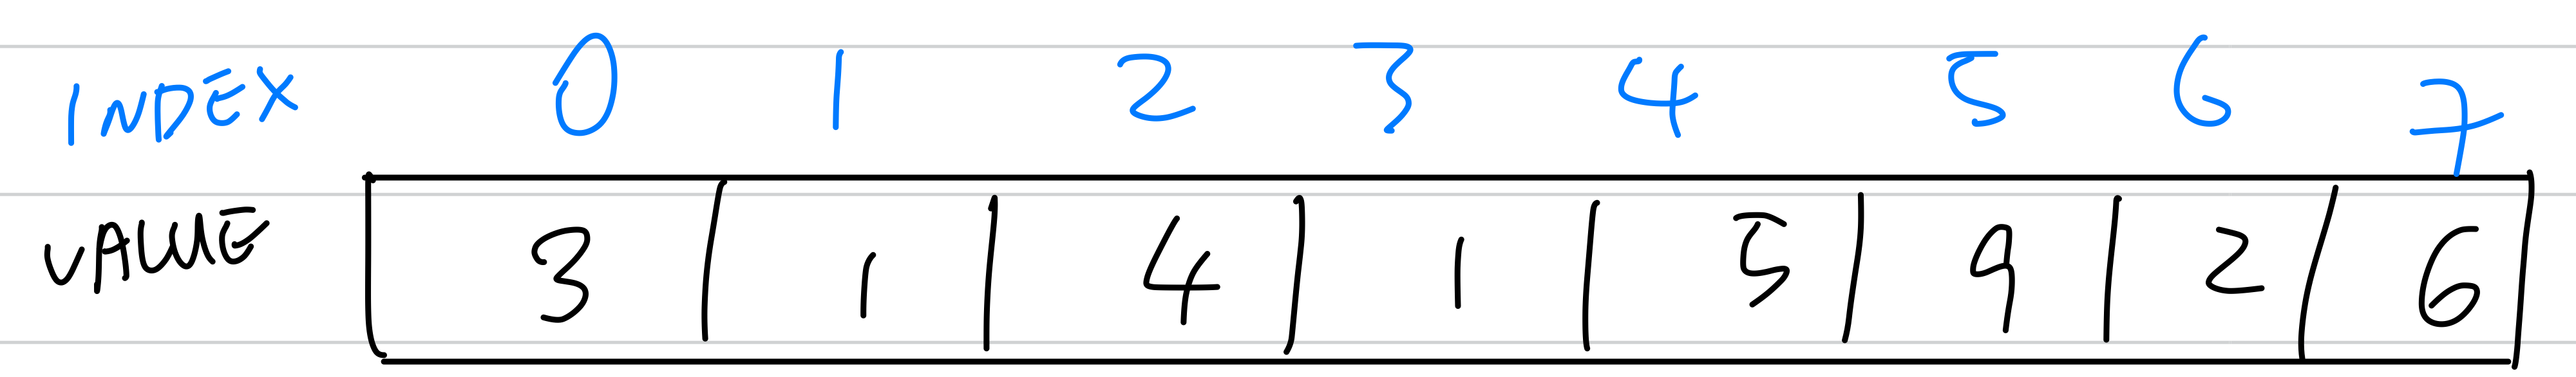
\includegraphics[width=12cm]{images/ch2-arrayindex.png}
\vspace{6mm}

There are two ways of initialising arrays. The first way is to hard-code the elements in the array. The length of the array is inferred by the number of elements given, and it cannot be extended afterwards.

\if\proglang1
\begin{lstlisting}
int[] x = {3,1,4,1,5,9,2,6};
\end{lstlisting}
\else
\begin{lstlisting}
int x[] = {3,1,4,1,5,9,2,6};
\end{lstlisting}
\fi

The second way is when you are not quite sure what the elements of the array are yet, but you must still supply the length of the array.

\if\proglang1
\begin{lstlisting}
int[] x = new int[8];
\end{lstlisting}
\else
\begin{lstlisting}
int x[8];
\end{lstlisting}
\fi

% Translated to Java end

\section{Loops}
\subsection{\texttt{for} loops}
Runs the body a specified number of times.

\begin{lstlisting}
int x[8] = {3,1,4,1,5,9,2,6};
int sum = 0;
for(int i = 0; i < 8; i++) { //loops i=0,1,2,3,4,5,6,7
    sum += x[i];
}
cout << sum << endl; //31
\end{lstlisting}

\begin{lstlisting}
int x[8] = {3,1,4,1,5,9,2,6};
int sum = 0;
for(int i = 7; i >= 0; i--) { //loops i=7,6,5,4,3,2,1,0
    sum += x[i];
}
cout << sum << endl; //31
\end{lstlisting}

\subsection{\texttt{while} loops}
Runs the body until the test is false.
\begin{lstlisting}
int x[8] = {3,1,4,1,5,9,2,6};
int sum = 0;
int i = 0;
while(i<8) { 
    sum += x[i]; //loops i=0,1,2,3,4,5,6,7
    i++;
}
cout << sum << endl; //31
\end{lstlisting}

\begin{lstlisting}
int x[8] = {3,1,4,1,5,9,2,6};
int sum = 0;
int i = 0;
while(i<8&&sum<10) { 
    sum += x[i];
    i++;
}
cout << sum << endl; //14
\end{lstlisting}

\subsection{\texttt{do while} loops}
Runs the body until the test is false. The body will run at least once.

\begin{lstlisting}
bool emergency = false;
do{
    printf("EMERGENCY\n"); //will be printed
}while(emergency);
\end{lstlisting}

\begin{lstlisting}
bool emergency = false;
while(emergency){
    printf("EMERGENCY\n"); //will not be printed
}
\end{lstlisting}

This example yields the same result with while loops because the test is true initially, allowing the loop to run at least once.

\begin{lstlisting}
int x[8] = {3,1,4,1,5,9,2,6};
int sum = 0;
int i = 0;
do { 
    sum += x[i]; //loops i=0,1,2,3,4,5,6,7
    i++;
}while(i<8);
cout << sum << endl; //31
\end{lstlisting}

\subsection{Infinite loops}

If the test case is always true (there is nothing in the loop to make the test false). The loop is an infinite loop\index{infinite loop}, where the loop will not terminate (until resources are used up), and the remaining parts of the program can never be run. In this example, EMERGENCY will be printed forever nonstop.

\begin{lstlisting}
bool emergency = true;
while(emergency){
    printf("EMERGENCY\n");
}
destroy_world(); //will not be run
\end{lstlisting}
\vspace{6mm}

\subsection{\texttt{break}}

\texttt{break} allows you to terminate the loop early.

\begin{lstlisting}
int x[8] = {3,1,4,1,5,9,2,6};
int sum = 0;
int i = 0;
while(i<8) { 
    sum += x[i];
    i++;
    if(sum >= 10) break;
}
cout << sum << endl; //14
\end{lstlisting}

\subsection{\texttt{continue}}

\texttt{continue} allows you to jump to the next iteration, skipping the rest of the current iteration early.

\begin{lstlisting}
int x[8] = {3,1,4,1,5,9,2,6};
int sum = 0;
int i = 8;
while(i>0) {
    i--;
    if(x[i] >= 5) continue;
    sum += x[i];
}
cout << sum << endl; //11
\end{lstlisting}

\subsection{Necessity of \texttt{break} and \texttt{continue}}

% Note that all for loops and do while loops can be written as a while loop.

% \begin{lstlisting}[basicstyle=\rmfamily]
% for(int i = 0; i < <target>; i++) <body> === 
% int i = 0; while(i < <target>) <body> i++;
% \end{lstlisting}

% \begin{lstlisting}[basicstyle=\rmfamily]
% do <body> while(<test>); === <body> while(<test>) <body>
% \end{lstlisting}

Note that the use of \texttt{break} and \texttt{continue} can be avoided by modifying the loop condition and using if statements respectively. 

In fact, plenty of other programming languages do not have \texttt{break} and \texttt{continue}. 

\section{2D arrays}

Don't have time to cover, there should be plenty of resources online on this topic.

\begin{lstlisting}
int x[3][] = {{1,4,7},{2,5,8},{3,6,9}};
cout << x[2][1] << endl; //6
\end{lstlisting}

\subsection{Nested loops}

\begin{lstlisting}
int x[3][] = {{1,4,7},{2,5,8},{3,6,9}};
sum = 0;
for(int i=0;i<3;i++)
    for(int j=0;j<3;j++)
        sum += x[i][j];
cout << sum << endl; //45
\end{lstlisting}

% Translated to Java 
\section{\if\proglang1 Methods \else ~functions \fi}

\if\proglang1 Methods \else ~functions \fi let you organize code better and reduce the amount of repeated code. You can define them by:

\if\proglang1
\begin{lstlisting}[language=,basicstyle=\rmfamily]
public static <return type> <name>(<arguments>){
    return <return value>;
}
\end{lstlisting}
\else
\begin{lstlisting}[language=,basicstyle=\rmfamily]
<return type> function(<arguments>){
    return <return value>;
}
\end{lstlisting}
\fi

For example, this \texttt{fact}\if\proglang1 method \else ~function \fi accepts an integer x, and returns another integer.
\if\proglang1
\begin{lstlisting}
public static int fact(int x){
    int y = 1;
    for(int i = 1; i <= x; i++){
        y *= i;
    }
    return y;
}
//What would happen if we input a negative number?
\end{lstlisting}
\else
\begin{lstlisting}
int fact(int x){
    int y = 1;
    for(int i = 1; i <= x; i++){
        y *= i;
    }
    return y;
}
//What would happen if we input a negative number?
\end{lstlisting}
\fi

This is how you use a\if\proglang1 method \else ~function \fi: 
You could call it by just supplying the argument.

\if\proglang1
\begin{lstlisting}
    System.out.println(fact(6)); //720
\end{lstlisting}
\else
\begin{lstlisting}
    cout << fact(6) << endl; //720
\end{lstlisting}
\fi

Alternatively, we usually would prefer saving the value returned for later use.

\begin{lstlisting}
    int x = fact(6); //720 is now stored in x
\end{lstlisting}

You could use the \texttt{\textbf{void}} keyword to indicate that a\if\proglang1 method \else ~function \fi does not have a return value. For \texttt{void}\if\proglang1 methods \else ~functions \fi, if there is no explicit \texttt{return;} statement, the\if\proglang1 method \else ~function \fi will automatically quit at the end of the\if\proglang1 method \else ~function \fi. 

\if\proglang1
\begin{lstlisting}
import java.util.Scanner;

public static void giveComment(int score){
    if(score >= 70){
        System.out.println("Good job.");
    }else if(score >= 40){
        System.out.println("You got a pass.");
    }else{
        System.out.println("You failed.");
    }
    //automatically quits here
}

public static void main(String args[]){
    Scanner scanner = new Scanner(System.in);  
    int s = scanner.nextInt();
    giveComment(s);
}
\end{lstlisting}
\else
\begin{lstlisting}
void giveComment(int score){
    if(score >= 70){
        printf("Good job.\n");
    }else if(score >= 40){
        printf("You got a pass.\n");
    }else{
        printf("You failed.\n");
    }
    //automatically quits here
}

int main(){
    int s;
    cin >> s;
    giveComment(s);
    //returning 0 is optional for some C/C++ compilers, it is implied it returns 0 normally
}
\end{lstlisting}
\fi

The main\if\proglang1 method \else ~function \fi is just a\if\proglang1 method \else ~function \fi with no arguments and an integer as a return value. The main\if\proglang1 method \else ~function \fi (specially recognized by the compiler) is the point of entry of the program, the program terminates when the main program returns, returning 0 indicates that there is no error, and returning other integers indicate otherwise.
\vspace{6mm}

Note that the giveComment\if\proglang1 method \else ~function \fi must be placed in front of the main\if\proglang1 method \else ~function \fi, or else the main\if\proglang1 method \else ~function \fi could not call the giveComment\if\proglang1 method \else ~function \fi as the\if\proglang1 method \else ~function \fi has not been defined by the time the compiler reads till the main\if\proglang1 method \else ~function \fi. 

% Translated to Java end